\chapter{Literature Review} \label{chapter:literaturereview}
In this section we describe some techniques used in NLP, trying to give an overview of the current state of art and what is necessary to train a language model.

\section{Natural Language Processing}
\alert{Communication and the sharing of knowledge is an essential part of human society. History has shown that the best way to transmit knowledge is in writing. It is not difficult for a person to learn to read and to understand the context in texts. For computers, this task is much more difficult. Natural Language Processing (NLP) is a subfield of Artificial Intelligence (AI) which deals with teaching computers to understand and interpret human language and has emerged in 1940. The initial need of NLP was the translation from one language into another which was used during the second world war. Nowadays it is widely used in health care, spam detection, sentiment and cognitive analysis. NLP also provides computers with the ability to read text, hear speech, and communicate with humans. Every person had contact with a NLP device at least once in their life. The best example everyone might know are personal assistants like Siri or Alexa. These are applications which work with NLP and have learned to communicate with humans and nearly seem humanely.\newline
Generally speaking, NLP breaks down language into shorter, more basic pieces, called tokens (words, periods, etc.) which get saved as vectorial representations. The technique of mapping words to real vectors is called word embedding. To understand the relationships of the tokens, the model gets trained by predicting some hidden part of the text using some other part of their surrounding text. One way to calculate the representations of the vectors is the method \textit{Word2Vec}. Until BERT has emerged, Word2Vec was the most common technique to create word embeddings. It is a two-layer neural network which processes text and turns it into a numerical form that can be understand by deep neural networks. Given enough data, Word2vec can make highly accurate guesses about a word’s meaning based on past appearances. Those guesses can be used to establish a word’s association with other words. The diference between Word2Vec and BERT will be covered in Section \ref{bert}}.

\section{Text Representation}
Text representation is a fundamental problem of NLP and necessary for preparing raw text as input for a language model. It aims to create a numerical representation of the unstructured text and make them mathematically computable. It is also called text vectorization or feature extraction.\newline
Texts cannot be processed by ML models directly. Tokenization is a method that transforms sequences of characters into a sequence of integers. As an example we can take the sentence: \newline

\centerline{"This is a cat."} 

A tokenization transforms this sentence into [‘This’, ‘is’, ‘a’, cat’]. Punctuations will be removed. This step is important to help the model understanding the meaning of a text. The model can
\begin{itemize}
	\item Count the number of words in the text
	\item Count the frequency of the word, that is, the number of times a particular word is present
\end{itemize} 

In modern LMs, tokenizers are trained together with the model to identify the best possible transformations, which can happen on both word and sub-word levels. The set of obtained tokens determines the vocabulary of an LM. If a word appears in the vocabulary of LM, it can be represented as a vector in the target space. Otherwise, a word is split into parts until each of them can be mapped to a set of tokens from the vocabulary. In the worst case, a word is split into individual letters. Such splitting may significantly reduce the quality of word embeddings in the vector space, thus reducing the quality of features extracted for the classification layers of a network. Therefore, it is essential either to select an LM whose vocabulary provides good coverage of the main terms used in an application domain or to extend the vocabulary of an LM with these terms and fine-tune it on domain-specific texts. 

The next chapters cover the most common techniques of text representation.

\subsection{One-Hot Encoding}
One-hot encoding is a type of representation were words in a document get converted in a V-dimension vector. When combining all, the result is a single document in the shape of a 2-D array as shown in the example below. In this example we assume that the document contains only the sentence \textbf{This is a cat.}:

\begin{table}[H]
	\centering
	\begin{tabular}{ll}
		\hline
		\textbf{Word} & \textbf{Vector Representation} \\ \hline
		This & [1, 0, 0, 0]\\ 
		is    & [0, 1, 0, 0]\\ 
		a & [0, 0, 1, 0]\\ 
		cat  & [0, 0, 0, 1]\\ \hline
	\end{tabular}
	\caption{One Hot Encoding Example}
	\label{tab:onehot}
\end{table}

Although it is very simple, one-hot encoding has the disadvantage of sparsity. Every single sentence creates a vector of n*m size where n is the length of sentence m is a number of unique words in a document and 80 percent of values in a vector is zero. Also each document is of a different length which creates vectors of different sizes. Later in chapter \ref{bert} it will be described that vectors of different sizes cannot be feed into the model.
As the last disadvantage one-hot encoding does not capture semantics. The actual meaning of a sentence should be observed in numbers which is not possible whith this technique as the example shows.

\subsection{Term Frequency - Inverse Document Frequency}
Term Frequency - Inverse Document Frequency (TF-IDF) is a statistical measure to determine how important a word is within a document. It determines not only how often a word appears in a single document, but also how often it appears in the entire document corpus. Very common words like "this" or "and" get a lower score, even though they occur often, because they are not important for the context of a document. This will be determined by comparing the occurrence of these words among the documents. This strategy is often used in NLP for text analysis. For example, in a failure analysis report, a word like failure would get a high score. By using other important words, the report could be automatically assigned to a certain failure type and thus classified. \\
TF-IDF for a word in a document is calculated by multiplying the term frequency and the inverse document frequency.

\begin{align}
	tf idf (t, d, D) &= tf(t, d) * idf(t, D)
\end{align}
Where
\begin{align}
	tf (t, D) &= log(1 + freq(t, d)) \\
	idf(t, D) &= log(N/count(d E D, t E d))
\end{align}

The term frequency \textit{tf} is either a simple count of instances a word appears in a document or it can be adjusted by taking the length of the document to account. The calculation can be seen in (2.3) where \textit{t} is the term and \textit{D} the document to analyse. The inverse document frequency \textit{idf} is determined accross the document corpus. The closer this metric is to zero, the more common a word is. The calculations can be seen in (2.4) where \textit{N} is the number of documents.

\subsection{Bag of Words}
Bag of Words is one of the most used text vectorizing techniques. It is a method for simplifying the representation of documents and the importance of the words they contain which is used in NLP and Information Retreivel (IR). Here the sentences in the documents are divided into their individual words and counted. The resulting object contains a list of the contained words and the number of their occurrences. It is called a “bag” of words, because any information about the order or structure of words in the document is discarded. The model is only concerned with whether known words occur in the document, not where in the document. We will describe the concept of bag-of-words with the following example: The below snippet contains the first few lines of the book "A Tale of Two Cities" by Charles Dickens.

\begin{table}[H]
	\centering
	\begin{tabular}{ll}
		\hline
			It was the best of times,\\
			it was the worst of times,\\
			it was the age of wisdom,\\
			it was the age of foolishness, \\
		 \hline
	\end{tabular}
	\caption{Example document for bag of words technique}
	\label{tab:bow}
\end{table}

In this example, each line will be treated as an individual document. The model vocabulary is containing the following 10 words:
\begin{itemize}
	\item “it”
	\item “was”
	\item “the”
	\item “best”
	\item “of”
	\item “times”
	\item “worst”
	\item “age”
	\item “wisdom”
	\item “foolishness”
\end{itemize}

Using this vocabulary, vector representations can be created for any document. For this purpose, a suitable scoring method must be chosen. The scoring method can be binary scoring or frequencies. Table \ref{tab:scoring1} is showing an example of the resulting vector representations for a document which contains all of the lines in our example.

\begin{table}[H]
	\centering
	\begin{tabular}{ll}
		\hline
		\textbf{Scoring Method} & \textbf{Resulting Vector Representation}                                         \\ \hline
		Binary & [1, 1, 1, 1, 1, 1, 1, 1, 1, 1] \\ \hline
		Frequencies & [4, 4, 4, 1, 4, 2, 1, 2, 1, 1] \\ \hline
	\end{tabular}
	\caption{Example of scoring methods for a document including the entire corpus}
	\label{tab:scoring1}
\end{table}

As a second example Table \ref{tab:scoring2} is showing the resulting vectors for a document which would include only the first two lines of our corpus in Table \ref{tab:bow}:

\begin{table}[H]
	\centering
	\begin{tabular}{ll}
		\hline
		\textbf{Scoring Method} & \textbf{Resulting Vector Representation}                                         \\ \hline
		Binary & [1, 1, 1, 1, 1, 1, 1, 0, 0, 0] \\ \hline
		Frequencies & [2, 2, 2, 1, 2, 2, 1, 0, 0, 0] \\ \hline
	\end{tabular}
	\caption{Example of scoring methods for a document including the first two lines}
	\label{tab:scoring2}
\end{table}

In comparison to one-hot encoding, the resulting vectors are of fixed size and can be feed into machine learning models. There is still the disadvantage of sparsity because the vectors can get very long.

\subsection{Word2Vec Architecture}
Word2vec is not a singular algorithm, it is a family of model architectures and optimizations that can be used to learn word embeddings from large datasets. The strength of Word2Vec lies in assigning similar vectors to words with similar meanings. With other methods like one-hot encoding, all the words in a vocabulary are independent of each other. With Word2Vec the embedding can be obtained using two methods (both involving Neural Networks): Skip Gram and Common Bag Of Words (CBOW).

\subsubsection{Common Bag of Words}
This method takes the context of each word as the input and tries to predict the word corresponding to the context. Considering the example \textit{Have a great day}, let the input to the Neural Network be the word, \textit{great}. The goal is to predict a target word \textit{day} using the single context input word \textit{great}. In the process of predicting the target word, the network learns the vector representation of the target word. Figure \ref{fig:cbow_network} shows the architecture of a simple CBOW model with one hidden layer where \textit{Wvn} is the weight matrix that maps the input \textit{x} to the hidden layer which is a V*N dimensional matrix. \textit{W`nv} is the weight matrix that maps the hidden layer outputs to the final output layer which is a N*V dimensional matrix. The hidden layer neurons just copy the weighted sum of inputs to the next layer.

\begin{figure}[H]
	\centering
	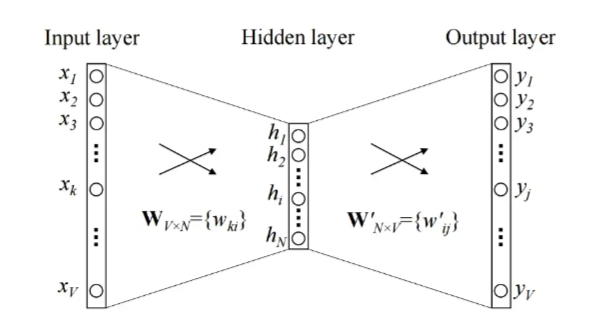
\includegraphics[width=0.9\textwidth]{figures/cbow_network.png}
	\caption{Simple CBOW Network with one hidden layer}
	\label{fig:cbow_network}
\end{figure}

The model in Figure \ref{fig:cbow_network} uses a single context word to predict the target word. The same calculations and predictions can be done by using multiple context words as an input and feed them into the hidden layer.

\subsubsection{Skip Gram}
The Skip Gram model is an alternative to the CBOW model and works the other way around. It uses the target word to predict the context and produces the representation of the tarked word during the process. An example of the model is shown in Figure \ref{fig:sgram_network}.

\begin{figure}[H]
	\centering
	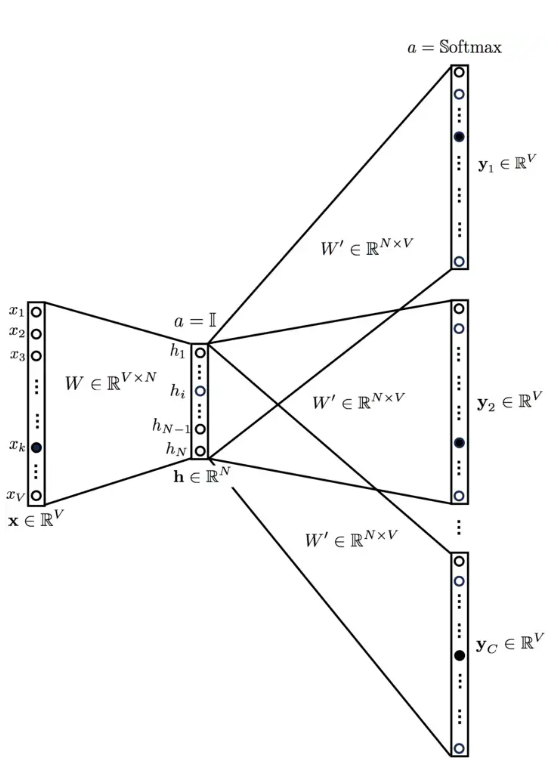
\includegraphics[width=0.6\textwidth]{figures/sgram_network.png}
	\caption{Simple CBOW Network with one hidden layer}
	\label{fig:sgram_network}
\end{figure}

When putting the target word into the network, the model outputs C probability distributions which means that for each context position, we get C probability distributions of V probabilities, one for each word.
\newline
In both cases, the models are using back propagation to learn.

\section{Masked Language Modelling}
Masked Language Modeling (MLM) is a learning technique which got introduced with the language model BERT in 2018. For this training method some tokens of the input sentence will get masked as in the example \textit{Today is a [MASK] day.} Before discussing the method in deep, we want to introduce the BERT model and the transformer architecture.

\subsection{Transformer} \label{chap:transformer}
The transformer in the field of NLP is a new architecture which is able to solve sequence-to-sequence tasks while handling dependencies in the text. Transformers basically consist of an encoder and a decoder. The encoder reads the input text and the decoder produces a prediction. Transformers work in small increments. In each step, an attention mechanism is applied to understand the relationships between the words in a sentence, regardless of their positions. Both encoder and decoder sections of transformer are a stack of six identical layers of multi-head attention and feed forward sublayers. The architecture is depicted in Figure \ref{fig:transformer}.

\begin{figure}[H]
	\centering
	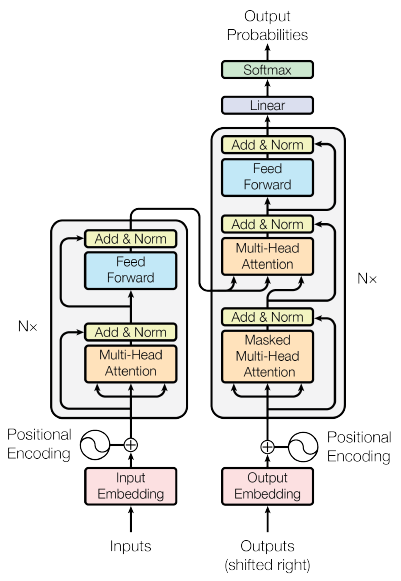
\includegraphics[width=0.5\textwidth]{figures/transformer_architecture.png}
	\caption{Transformer Architecture}
	\label{fig:transformer}
\end{figure}

The encoder maps an input sequence of symbol representations \textit{x1, ... , xn} to a sequence of representations \textit{z = (z1, …, zn)}. Given \textit{z}, the decoder then generates an output sequence \textit{(y1, …, ym)} of symbols one element at a time. Each layer has an output of dimension 512.

\subsection{Evolution of Language Models}
It has always been difficult to teach a computer to really understand natural language. While they are capable of processing and storing large amounts of data, they lack language context. This problem continued until NLP became popular in the Artificial Intelligence field. NLP enables computers to read, analyze, interpret and gather information from long texts and single written words. In contrast to before without NLP, meaning and sense of texts can now be determined. In the beginning, a separate model was developed and used for each of these tasks. Since the development of BERT in 2018, this has changed. Engineers are now able to use a single model to handle the most common NLP tasks such as Classification, Sentiment Analysis or Question Answering. The timeline depicted in Figure \ref{fig:timeline} shows the evolution of NLP models from \textit{Bag OF Words} until \textit{BERT}.

\begin{figure}[H]
	\centering
	\includegraphics[width=1\textwidth]{figures/timeline_NLP.PNG}
	\caption{Timeline of Model evolution in NLP.}
	\label{fig:timeline}
\end{figure}

The following sections will briefly describe all of the mentioned models to cover all the important topics which will be discussed in this paper and to prepare for the technical details of BERT.

\subsection{BERT} \label{bert}
BERT  stands  for  Bidirectional Encoder Representations from Transformers. It makes use of a transformer and an attention mechanism that learns contextual relations between words or sub-words in a text. 
A Transformer usually includes two separate mechanisms, an encoder that reads the text input and a decoder that produces a prediction for the task, which got already introduced in chapter \ref{chap:transformer}. For producing a language model, only the encoder mechanism is necessary. The BERT model was developed by Google researchers in 2018 and is already pre-trained using a combination of masked language modeling objective and next sentence prediction on a large corpus. The original BERT model comes in two sizes: BERT-base (trained on BooksCorpus: ~800 million words) and BERT-large (trained on English Wikipedia: ~ 2,500 million words). 
In contrast to previous language models which looked at a text sequence either from left to right or combined left-to-right and right-to-left training, BERT is using the bidirectional approach. The paper’s results show that a language model which is bidirectionally trained can have a deeper sense of language context and flow than single-direction language models. To do this, the authors introduced a new technique which is called Masked Language Modelling. This objective randomly masks 15\% tokens from an input sequence during training. The model has to predict the original token based on the context. Out of these 15\%, the algorithm exchanges 80\% of the tokens with the [MASK] token, 10\% with any random word and the other 10\% remain the same word. The second pre-training technique introduced in BERT is Next Sentence Prediction that takes in a sentence-pair input, replaces the second input sentence with a random sentence for 50\% of the training steps, and trains on the sentence pairs to learn sentence relationships. \newline  
The input to BERT's encoder is a sequence of tokens previously converted into vectors. Later, these tokens can be processed in the neural network. In order to be able to do this, a few steps must first be carried out:
\begin{enumerate}
	\item CLS and SEP tokens at the beginning and end of each sentence
	\item Segment embeddings for each token to distinguish between sentences.
	\item Position embeddings for each token to identify the position in a sentence.
\end{enumerate}
These three steps are depicted in Figure \ref{fig:bert_tokenizing}.

\begin{figure}[H]
	\centering
	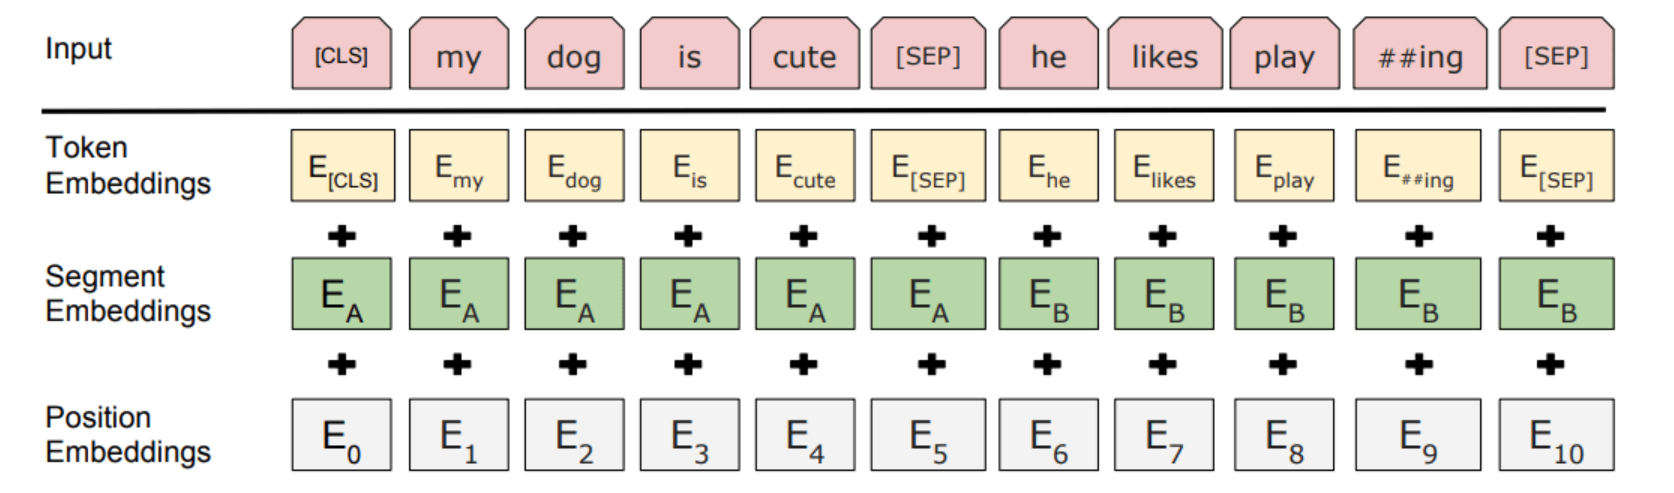
\includegraphics[width=1\textwidth]{figures/bert_tokenizing.png}
	\caption{Embeddings of Text Input with BERT.}
	\label{fig:bert_tokenizing}
\end{figure}

BERT is optimized to either get a single text sentence or a pair of text sentences as input. In the case of two sentences, each token in the first sentence receives embedding A, and each token in the second sentence receives embedding B as visible in Figure \ref{fig:bert_tokenizing}. As each layer in the transformer architecture produces an ouptut of dimension 512, the supported sequence length of BERT is also 512 tokens. \newline

The training of the BERT language model is divided into pre-training and fine-tuning. The pre-training process starts with next sentence prediction tasks followed by MLM tasks. For the NSP, 50\% of the time the sentence B is replaced with a random sentence. After the pre-training, the fine-tuning process follows which includes an added classification layer. In particular, the fine-tuning process is aimed at certain NLP downstream tasks. During fine-tuning only batch size, learning rate and the number of training epochs are adapted. All other hyperparamethers stay the same as during pre-training. The two training processes are depicted in Figure \ref{fig:bert_training}\alert{ \cite{Devlin}}.

\begin{figure}[H]
	\centering
	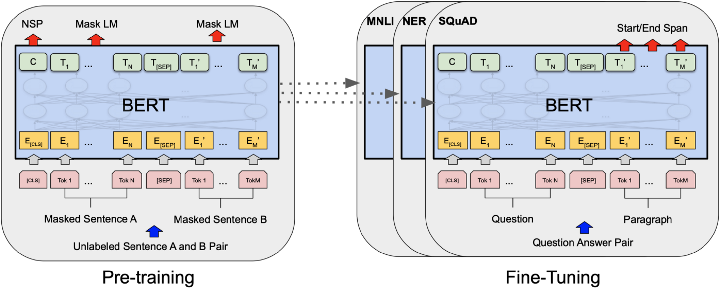
\includegraphics[width=1\textwidth]{figures/bert_training.png}
	\caption{Pre-Training and Fine-Tuning Process of BERT}
	\label{fig:bert_training}
\end{figure}



\subsubsection{Difference between BERT and Word2Vec}
Word2Vec is contex-independent, so it only has a numeric vector to represent a word. If a word has several meanings, these are combined into a vector.

BERT, on the other hand, is context-dependent and thus allows multiple numeric vectors as a representation for a word, depending on the context in which the word occurs.

An example of the difference is the word bank, which can appear in a financial context as well as in a beach or park context. Word2Vec will always generate the same vector for this word and can therefore lead to an inaccurate representation. BERT can distinguish the two different semantic meanings and thus also generate two different vectors.

\begin{enumerate}
	\item The next difference is that Word2Vec doesn't care about the position of words in a sentence. BERT, on the other hand, uses the position (index) of a word as input for calculating the vector.
	\item Word2Vec only needs one word as input and delivers a vector as output. BERT, on the other hand, needs an entire sentence as input because it needs the context of the sentence to calculate the vector.
	\item Word2Vec can have problems if a word is not stored in the vocabulary and no vector can be generated. BERT can also create a vector for subwords that are not stored in the vocabulary and is therefore not limited by the vocabulary.
\end{enumerate}

